\section{Scopo del tirocinio}

Lo scopo di questo tirocinio è la realizzazione di nuovi materiali ibridi potenzialmente utilizzabili per lo strato fotoattivo di celle fotovoltaiche orgaiche di tipo \emph{bulk heterojunction}. In particolare verranno preparati nanocristalli di CdSe modificati con poli(3-esiltiofene). 

Il poli(3-esiltiofene) non verrà utilizzato tal quale per disperdere le nanoparticelle, bensì verrà funzionalizzato con gruppi leganti nei confronti del CdSe allo scopo di contrastare la tendenza delle \emph{NPs}\footnoteremember{NPs}{{\descriptionlabel{NPs}} nanoparticelle} all'aggregazione ed alla separazione delle fasi.

Come viene schematizzato in~\ref{fig:leganti} i gruppi leganti possono essere inseriti in varie posizioni sul polimero: nelle catene laterali, su entrambe le terminazioni, in un blocco di polimero legante non coniugato o solamente su una delle due terminazioni.
\begin{figure}
\centering{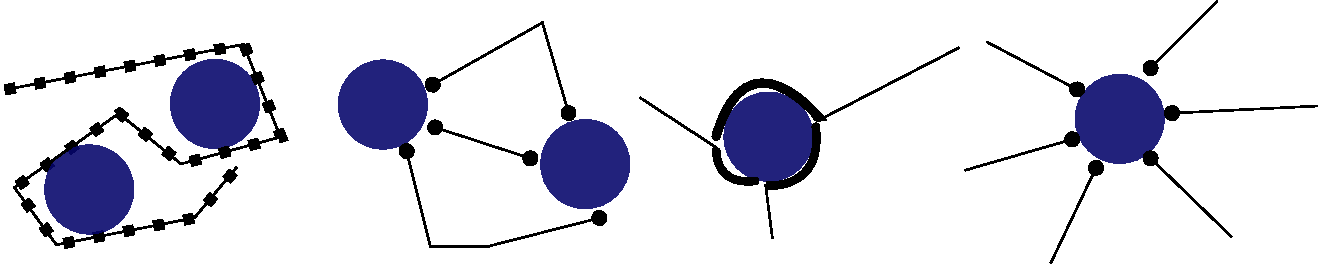
\includegraphics[width=.8\textwidth]{Immagini_Tesi/leganti.pdf}}
\caption{\footnotesize{Le posizioni in cui possono essere inseriti gruppi leganti sul polimero semiconduttore.}
\label{fig:leganti}}
\end{figure}
In questo lavoro è stata presa in considerazione l'ultima di queste possibilità, ossia la singola terminazione legante. Infatti le prime due possibilità sono da escludersi perché porterebbero alla formazione di materiali reticolati non plastici (la plasticità è uno dei punti di forza del fotovoltaico organico ed ibrido organico-inorganico). La terza opzione è utilizzabile ma inserisce nell'interfaccia polimero-nanoparticella un secondo tipo di polimero che rischia di agire da isolante.

Tra i molti gruppi leganti riportati in letteratura per il CdSe ( tioli, ammine, acidi carbossilici, acidi fosfonici, piridine sostituite in para ed altri ) in questo lavoro di tesi verrà realizzata per la prima volta una miscela NPs\footnoterecall{NPs} di CdSe - politiofene monoterminato con un gruppo fosfonico. Come si può osservare nella~\ref{fig:pol-finale} l'altra terminazione del polimero sarà un gruppo allile.
\begin{figure}
\centering{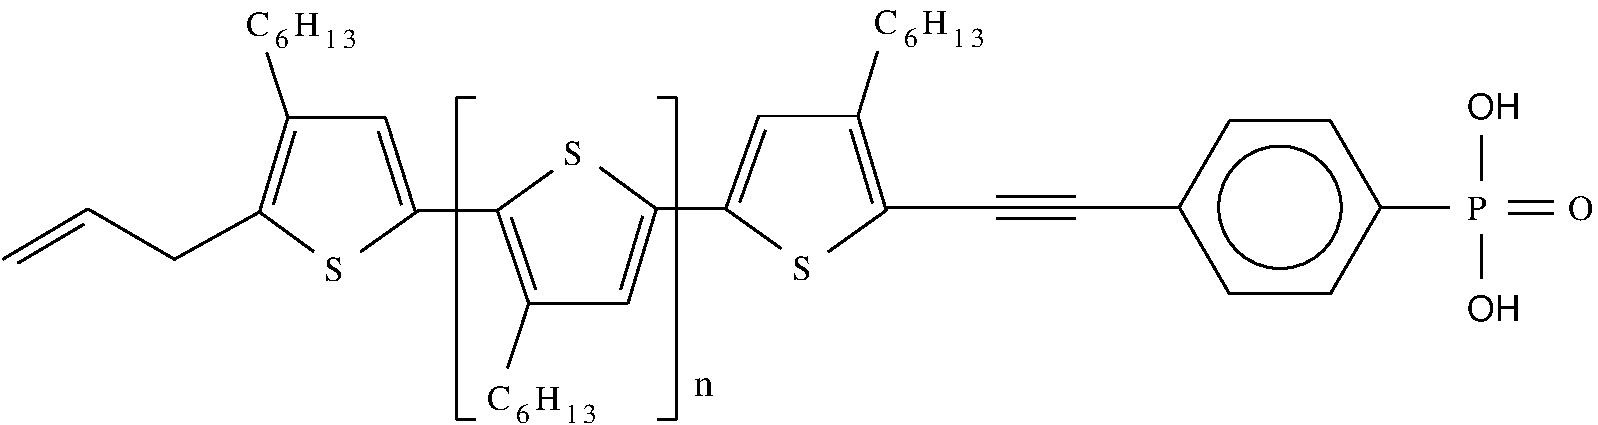
\includegraphics[width=1\textwidth]{Immagini_Tesi/pol-finale.pdf}}
\caption{\footnotesize{Il polimero sintetizzato completo di terminazione legante.}
\label{fig:pol-finale}}
\end{figure}
